\section{Advanced Topics}
\subsection{Theory}
\textbf{$p$-Norm Robustness:} For a multi-class classifier $f$, the goal of adversarial example perturbation is to find a perturbation $\eta$ given a pattern $x$ s.t. $f(x+\eta)\neq f(x) \; \text{s.t.} \; \|\eta\|_p \leq \epsilon$

For $p=2$ and a linear model with weight vectors $w_i$, we have $f(x)=\arg\max_if_i(x), \; f_i=w_i^\top x + b_i$. For binary classification, the optimal perturbation is then given by $\eta \propto \operatorname{sign}(f_1(x)-f_2(x))(w_2-w_1)$. This generalizes to  $m>2$ classes ($f(x)=1$ w.l.o.g.) by finding most easily confusable class: $\eta = \arg \min_{i>1}\frac{f_1(x)-f_i(x)}{\|w_1-w_i\|_2^2}(w_i-w_1)$\\

\textbf{Linearization:} Suggested in DeepFool: leverage the linear case to \emph{linearize} a nonlinear model and iteratively find an adversarial perturbation. For $m=2$ one iterates solving the problem $\arg\min_{\Delta \eta} \|\Delta \eta\|_2, \; \text{s.t.} \; (\nabla f_1(x) - \nabla f_2(x))^\top \Delta \eta < f_1(x)-f_2(x)$, with $f_1(x)-f_2(x)$ being the margin. This can be generalized to $p$-norms.\\
\textbf{Robust Training:} Loss is extended to neighborhoods of training points: $\ell(f(x), y)\mapsto \max_{\eta: \|\eta\|_p\leq \epsilon} \ell(f(x+\eta), y)$
which yields a minimax problem, where adversary picks worst perturbation $\eta$ an learner picks best parameter $\theta$ in response. One can solve inner loop maximization via \emph{projected gradient ascent}. For $p=2$: $\eta^{t+1}=\epsilon\Pi\left[\eta^t + \alpha\nabla_x\ell(f(x+\eta^t),y)\right],\;\Pi[z]\equiv\frac{z}{\|z\|_2},$ for $p=\infty: \; \eta^{t+1}=\epsilon\Pi\left[\eta^t + \alpha \operatorname{sign}(\nabla_x \ell(f(x+\eta^t), y))\right],\; \Pi[z]\equiv \frac{z}{\|z\|_{\infty}}$.

A practical method is Fast Gradient Sign Method (FGSM), which performs one iteration of $\|\cdot\|_\infty$-projected gradient descent: $\eta = \epsilon \operatorname{sign}(\nabla_x\ell(f(x),y)$, modifying the pixels by $\pm \epsilon$ depending on the sign of $\pd{\ell}{x_i}$ per pixel. FGSM results in $\approx 2\times$ overhead compared to standard training.

\subsection{Adversarial Attacks}
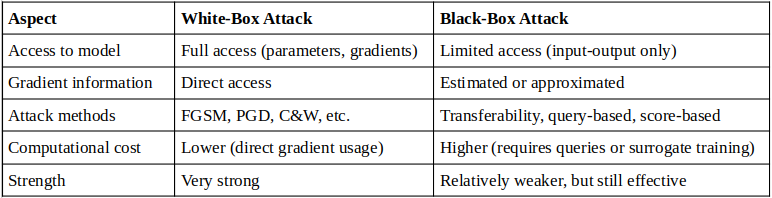
\includegraphics[scale =0.25]{contents/imgs/attack_types_new.png}

\textbf{Grey-box}: partial knowledge of target model, which could include some knowledge such as model architecture, training data, setup and ouputs, but does not have access to the exact model parameters (weights and biases) or gradients.

\textbf{Targeted vs Untargeted:}
\begin{itemize}
    \item \textbf{Untargeted}: aim to fool model such that output is anything different from the correct label
    \item \textbf{Targeted}: aim to fool model to return target label of the attacker's interest
\end{itemize}

\textbf{Types of Attacks:}
\begin{itemize}
    \item \textbf{Gradient-based:} for white-box setting by solving either targeted or untargeted adversarial objective (e.g. FGSM and PGD)
    \item \textbf{Optimization-based:} achieve adversarial objective while minimize perturbation size (e.g. Carlini\& Wagner attack)
    \item \textbf{Transferability-Based:} usually for black-box and grey-box; trains surrogate model $\implies$ generate adversarial examples based on the surrogate using optimization-based methods $\implies$ applied to target model
    \item \textbf{Query-based:} Usually for the black-box; if attacker can query the black-box model and observe its outputs (predictions or confidence scores), they can iteratively approximate gradients using optimization-based methods. Gradients can be estimated using \emph{finite differences}: $\pd{J}{x_i}\approx \dfrac{J(x+\delta e_i)-J(x)}{\delta}$
\end{itemize}
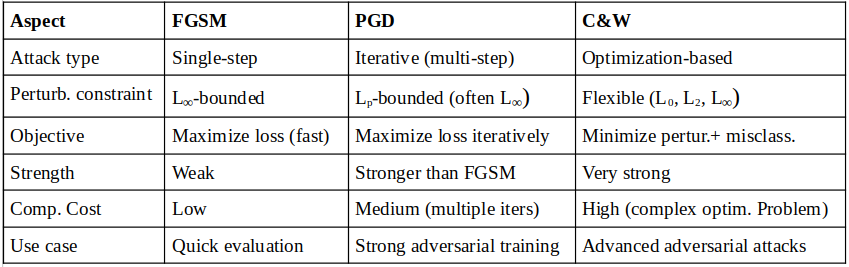
\includegraphics[scale =0.17]{contents/imgs/attacks_new.png}
\textbf{FGSM:} $x_{adv}=x+\epsilon \cdot \operatorname{sign}(\nabla_x J(\theta, x, y))$, where \(x:\) original input, \(\epsilon:\) perturbation magnitude (small scalar value), \(\nabla_x J(\theta, x, y)\) gradient of loss; FGSM is a special case of PGD with a single step\\
\textbf{PGD:} $x_{adv}^{(t+1)} = \operatorname{Proj}_{\mathcal{B}_\epsilon(x)}(x_{adv}^{(t)} + \alpha \cdot \operatorname{sign}(\nabla_x J(\theta, x_{adv}^{(t)}, y)))$, where \(\operatorname{Proj}_{\mathcal{B}_\epsilon(x)}\) projects adversarial examples back into the \(\epsilon\)-ball centered at \(x\).\\
\textbf{Carlini \& Wagner:} minimize \(\|x_{adv}-x\|_p + c\cdot f(x_{adv})\), where \(\|x_{adv}-x\|_p\) is perturbation size e.g. $L_2$ norm, c: regularization constant balancing perturbation size and attack success, \(f(x_{adv})\): function that ensures \(x_{adv}\) is misclassified (often \(f(x_{adv})\leq 0\) if attack succeeds). Then use optimization algorithm such as SGD or Adam to search for optimal \(x_{adv}\)

\subsection{Other Adversarial Attacks}
\begin{itemize}
    \item \textbf{Backdoor Attacks:} \emph{training-time} attack where an adversary injects hidden "backdoor" patterns into the training dataset. The model behaves normally on clean inputs but produces targeted outputs when presented with inputs containing the backdoor trigger
    \item \textbf{Privacy Inference Attacks:} \emph{test-time} attack where an adversary exploits the model's predictions to infer sensitive information about the training data e.g. \emph{Membership Inference} (determining whether data point was used during model training), \emph{Attribute Inference} (recovering specific attributes of the input data e.g. gender, age, private features)
    \item \textbf{Model Extraction Attacks:} adversary attempts to replicate or approximate the target model by querying it repeatedly and analyzing the outputs to reconstruct the model's behavior
    \item \textbf{Model Inversion Attacks:} \emph{test-time} attack where adversary uses the model's output predictions to reconstruct the input features, potentially revealing private or sensitive data
\end{itemize}

\subsection{Adversarial Defense}
\begin{itemize}
    \item \textbf{Denoising based methods:} attempt to use conventional image/signal processing techniques, GANs, autoencoders, or some generative approaches to erase the adversarial perturbations placed on the input samples
    \item \textbf{Randomization based methods:} based on random transformation or regularization with motivation that randomizing adversarial effects introduced in adversarial examples could potentially make DNNs more robust to them
    \item \textbf{Adversarial training based methods:} aim to improve robustness of DNNs by training them with adversarial examples. Motivation: adversarial examples can be considered scarce data residing near the true decision boundary. Including such samples in the training process will enable the models to learn more specific decision boundaries that take these outliers into consideration
\end{itemize}
Denoising-based easily bypassed by optim.-based approaches; randomization-based have been proven to be exploiting \emph{obfuscated gradient} which gives a false sense of security and can be easily compromised by adv. examples generated through Expectation over Transformation (EoT). \textbf{Adversarial training has been the most robust defense method}